\section{Actor basics}
\begin{frame}
\frametitle{Brief history}
\begin{itemize}
\item C. Hewitt et al. '73 onward: first theory of actor model, operational semantics, axioms
\item W. Clinger '81: proved unbounded nondeterminism property
\item G. Agha '85: formalization of semantic model
\item Theoretical/Practical research by MIT, CalTech, industry, etc.
\item Recent resurgence (strong relevance to distributed/cloud computing)
\end{itemize}
\end{frame}

\begin{frame}
\frametitle{``A Model of Concurrent Computation in Distributed Systems``}
\begin{itemize}
\item actors encapsulate computation (technically at any level)
\item an actor may only send messages to actors it knows by name
\item an (idling) actor receiving a message will accept it and execute the computation defined within, resulting in the possible actions:
	\begin{itemize}
	\item sending new messages
	\item creating new actors
	\item updating its local state
	\end{itemize}
\item an actor can only influence its own local state
\end{itemize}
\textrightarrow "self-contained, autonomous, interactive, asynchronously operating components" [Karmani, Agha]
\end{frame}

\begin{frame}
\frametitle{Example structure}
\begin{figure}
\centerline{
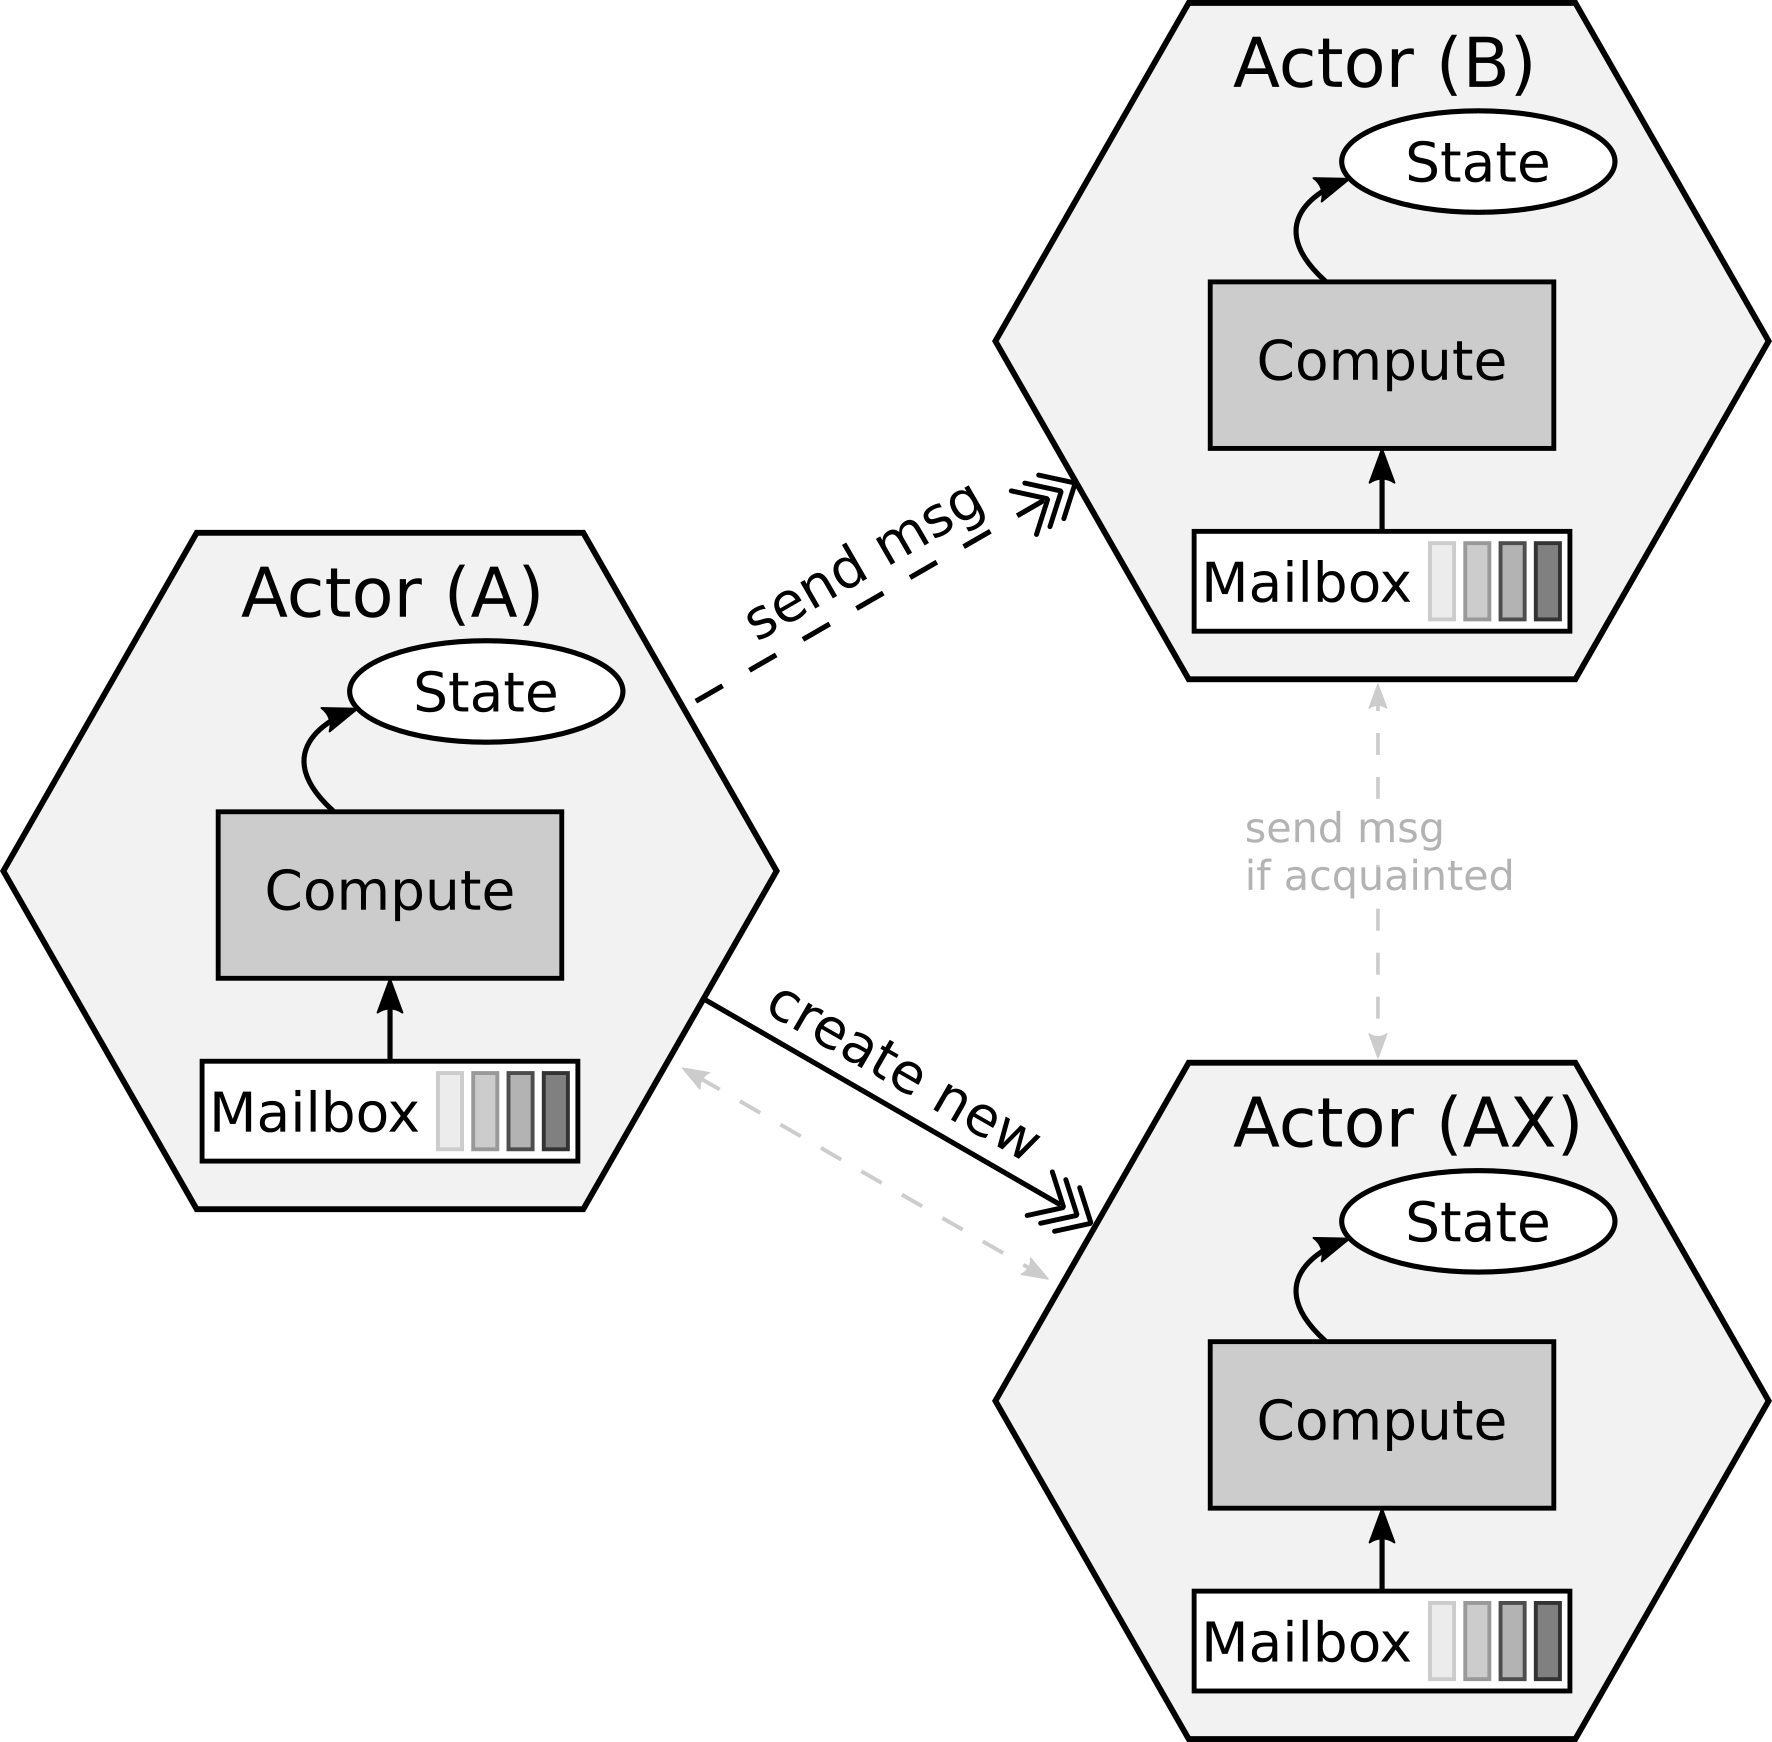
\includegraphics[width=0.6\textwidth]{actorsExample2}
}
\caption{Any actor may send messages to other known actors, create new actors or update its own state.}
% A label to allow refering to this figure in the text.
\label{Actors}
\end{figure}
\end{frame}

\begin{frame}[fragile]
\frametitle{Hello ...}
\begin{lstlisting}[language=C++, caption=sample code, frame=single, breaklines]
[includes, usings]

behavior pong(event_based_actor* self, string selfname) {
  return {
    //if the message contains a string, proceed
    [=](const string& what) -> string {
      aout(self) << selfname << ": " << what << endl;
      // reply Pong
      return string("Pong!");
    }
  };
}
\end{lstlisting}
Specify behavior
\end{frame}

\begin{frame}[fragile]
\frametitle{Hello ...}
\begin{lstlisting}[language=C++, caption=sample code, frame=single, breaklines]
void ping(event_based_actor* self, const actor& buddy, string selfname) {
  // send Ping to buddy (timeout for reply = 10s)
  self->request(buddy, std::chrono::seconds(10), "Ping!").then(
    //if the message contains a string, proceed
    [=](const string& what) {
      aout(self) << selfname << ": " << what << endl;
	  //if reply is as expected, restart ping again
	  if(what.compare("Pong...") == 0)
		  ping(self, buddy, selfname);
    }
  );
}
\end{lstlisting}
Specify actions
\end{frame}

\begin{frame}[fragile]
\frametitle{... World!}
\begin{lstlisting}[language=C++, caption=sample code, frame=single, breaklines]
int main() {
  [caf setup]
  // create a new actor that calls 'pong()'
  auto actor_B = system.spawn(pong, "B");
  // create another actor that calls 'ping(actor_B)';
  auto actor_A = system.spawn(ping, actor_B, "A"); }
\end{lstlisting}
Spawn actors and start something
\begin{lstlisting}[frame=single, breaklines]
B: Ping...
A: Pong...
B: Ping...
A: Pong...
B: Ping...
A: Pong...
[...]
\end{lstlisting}
Output
\end{frame}